\documentclass{beamer}

\usepackage{graphicx}
\graphicspath{ {./figures/} }

\title{COMP 354 - Summer 2021 \\ ETERNITY Calculator Project Organization Summary}
\author{Team I}
\date{} %remove date

\begin{document}
\maketitle

\section{Introduction} % doesn't show in all themes

\begin{frame}
\frametitle{Initial Project Meeting}
    \begin{itemize}
        \item Deciding the technology and language for ETERNITY \pause
        \item Breakdown of team members' skills, tasks and responsabilities \pause
        \item Organization of future meetings and communication
        \begin{itemize}
            \item Discord
        \end{itemize}
    \end{itemize}

    % maybe mention the math functions, how we each took one and did our research for implementing it.

\end{frame}

\begin{frame}
\frametitle{Initial Project Meeting}
    Breaking the project down into sub-tasks and task allocation based on skills and knowledge.
    \begin{itemize}
        \item Lead/ project GitHub Repository organizer 
        \item Documentation
        \item Fullstack Developer
        \item Backend Developer
        \item Frontend Developer
        \item Communication and resources
    \end{itemize}

\end{frame}

% This frame is optional, consider removing
\begin{frame}
\frametitle{Roles}
    \textbf{Lead/ project repository:}
    Robert \\
    \textbf{Documentation:}
    Xavier, Sobhan \\
    \textbf{Fullstack:}
    Chelsie \\
    \textbf{Backend:}
    Elijah \\
    \textbf{Frontend:}
    Michael \\
    \textbf{Communication and resources:}
    Hao mei \\
    \textbf{Major present:}
    Michael \\
    \textbf{Minor presenter:}
    Robert \\
\end{frame}

\section{Development Process}

\begin{frame}
    \frametitle{Interview Process}
    \begin{itemize}
        \item Funnel Strategy 
        \begin{itemize}
            \item General questions leading into more specific questions related to the ETERNITY calculator. \pause
        \end{itemize}

        \item Semi-structured \& Linear Progression
        \begin{itemize}
            \item Tried to ask some follow-up sub-questions based on the response to get more information \pause
            \item General questions to increasingly more specific questions (Funnel Strategy) \pause
        \end{itemize}
        \item 5 questions per team member
        \begin{itemize}
            \item 10 General questions
            \item 25 Specific questions
        \end{itemize}
    \end{itemize}
\end{frame}

\begin{frame}
    \frametitle{GitHub Repository}
    Not just for code version control.
    \begin{itemize}
        \item Issue tracking
        \item Kanban board linked to current issues
        \item Documentation
    \end{itemize}
\end{frame}

\begin{center}
\begin{frame}
    \frametitle{GitHub Repository - Issues}
    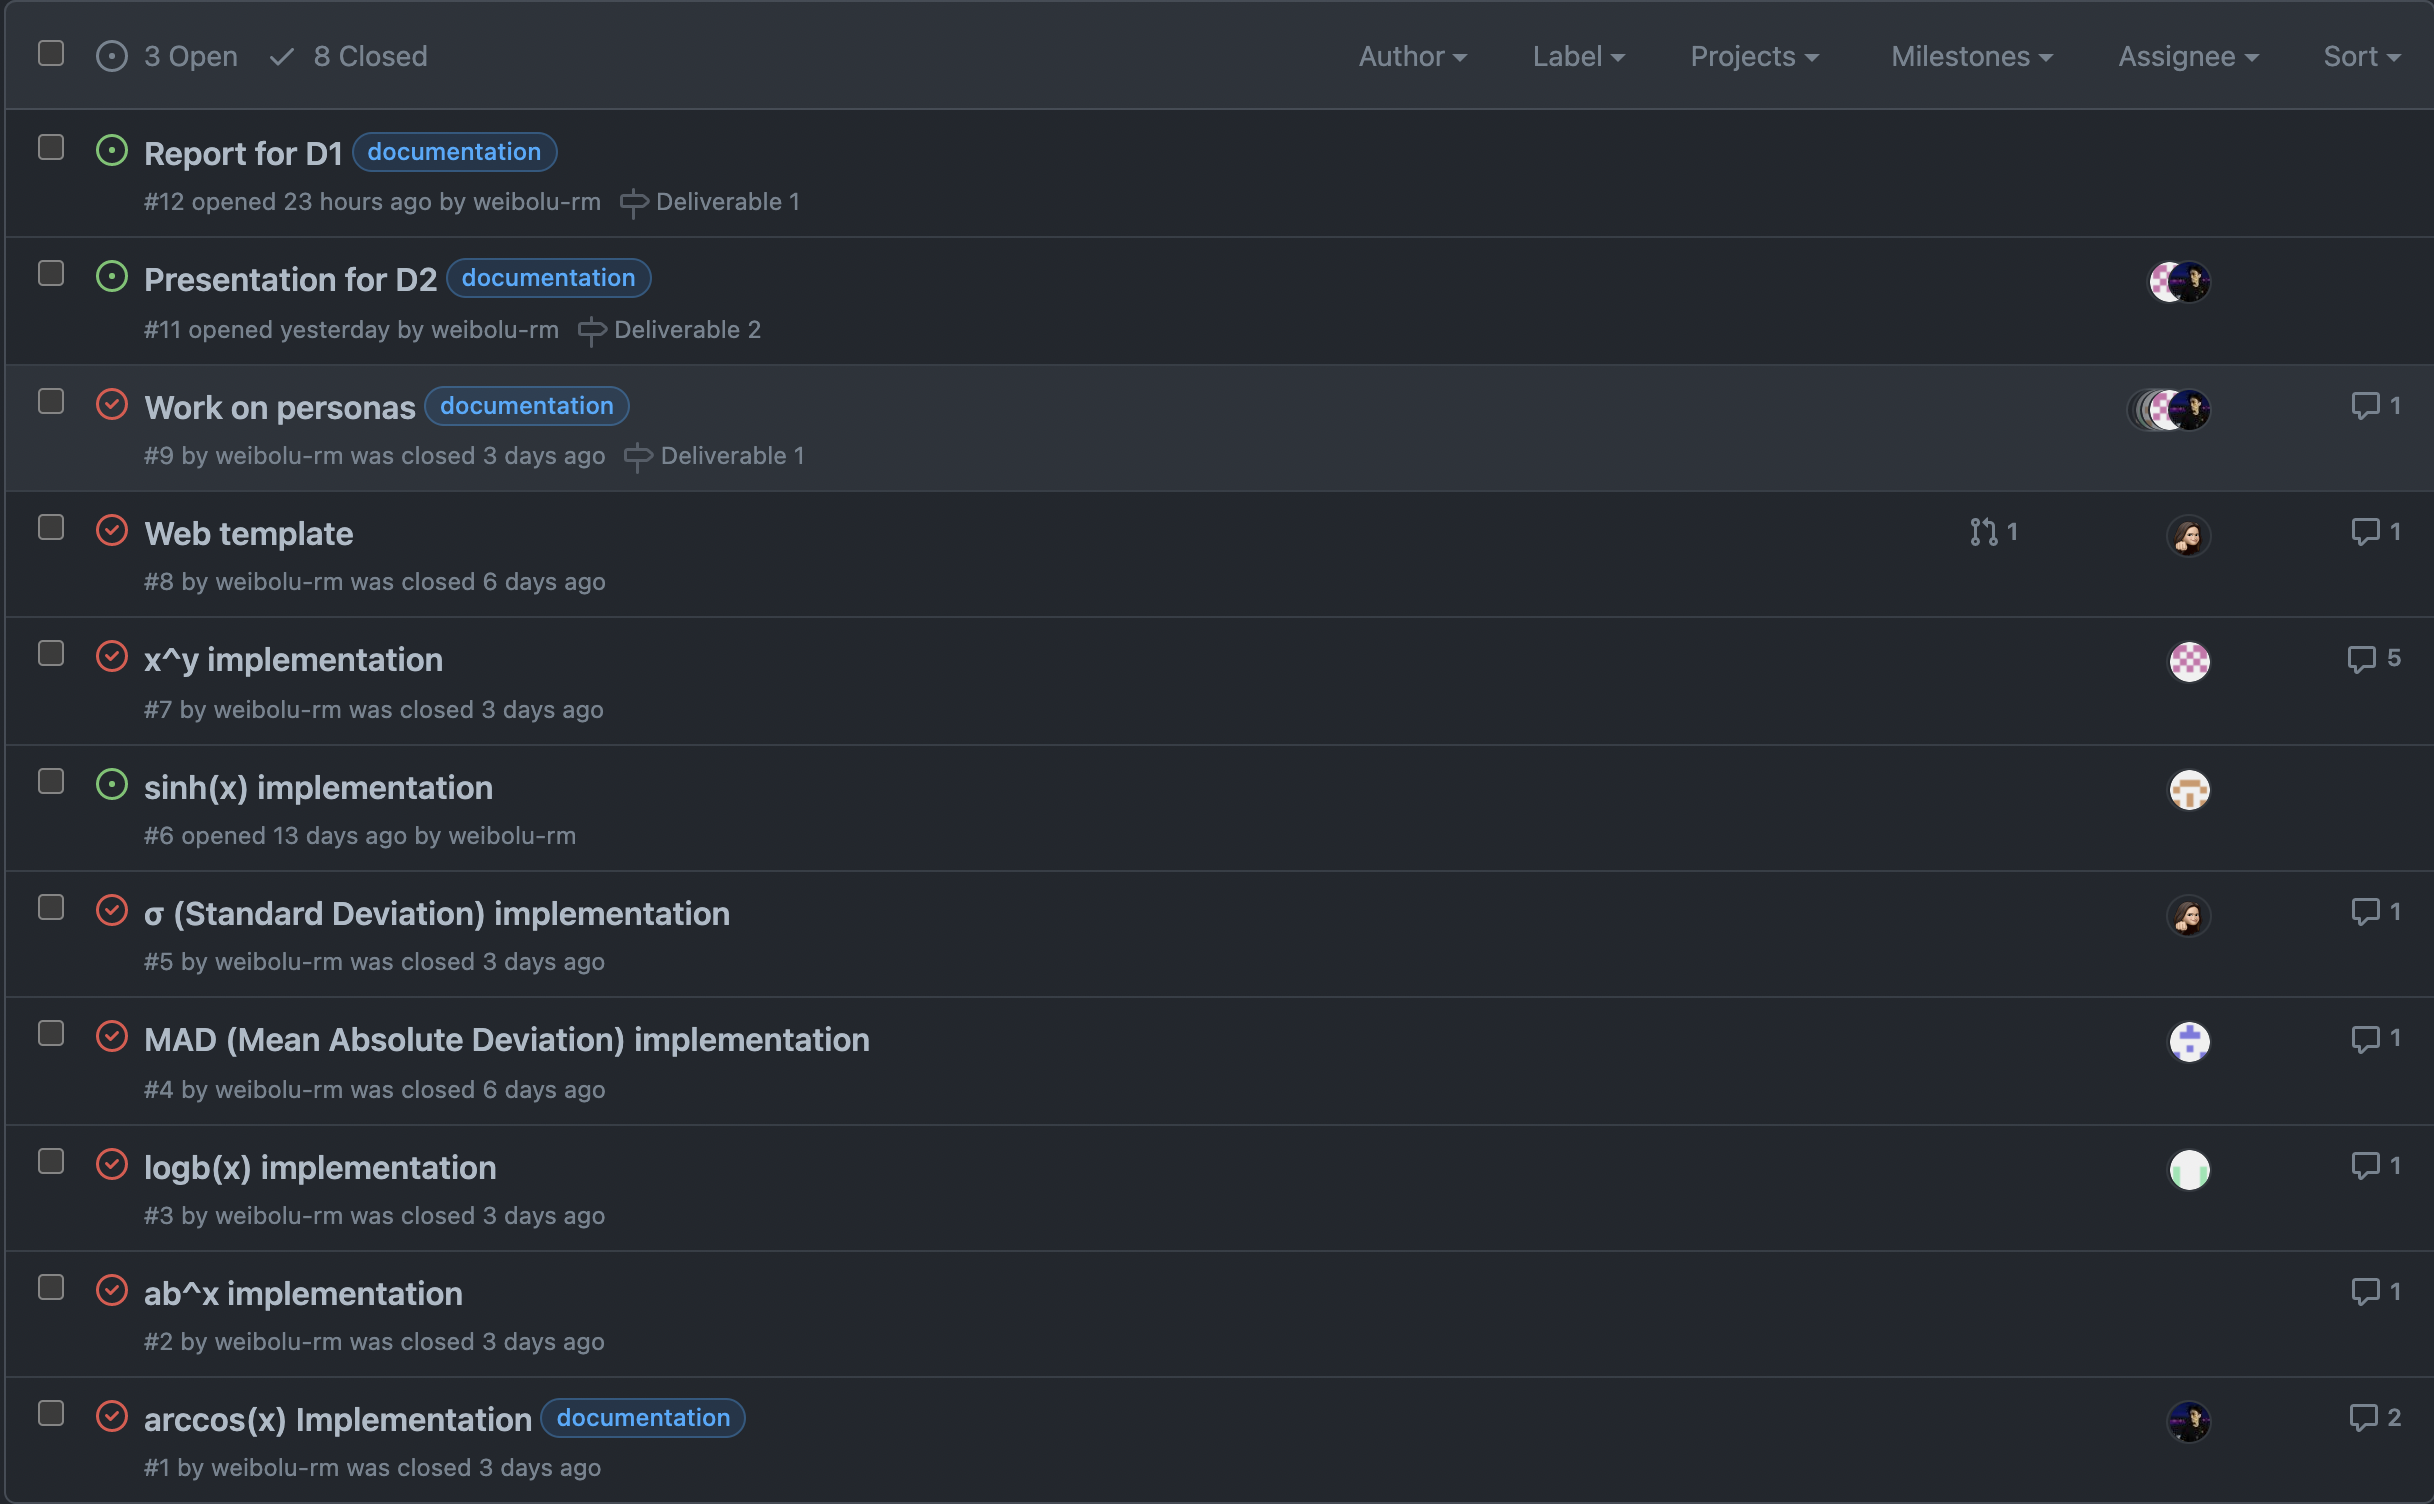
\includegraphics[width=\linewidth]{issues.png}
\end{frame}

\begin{frame}
    \frametitle{GitHub Repository - Kanban board}
    \includegraphics[height=.8\textheight]{board.png}
\end{frame}

\begin{frame}
    \frametitle{GitHub Repository - Documentation}
    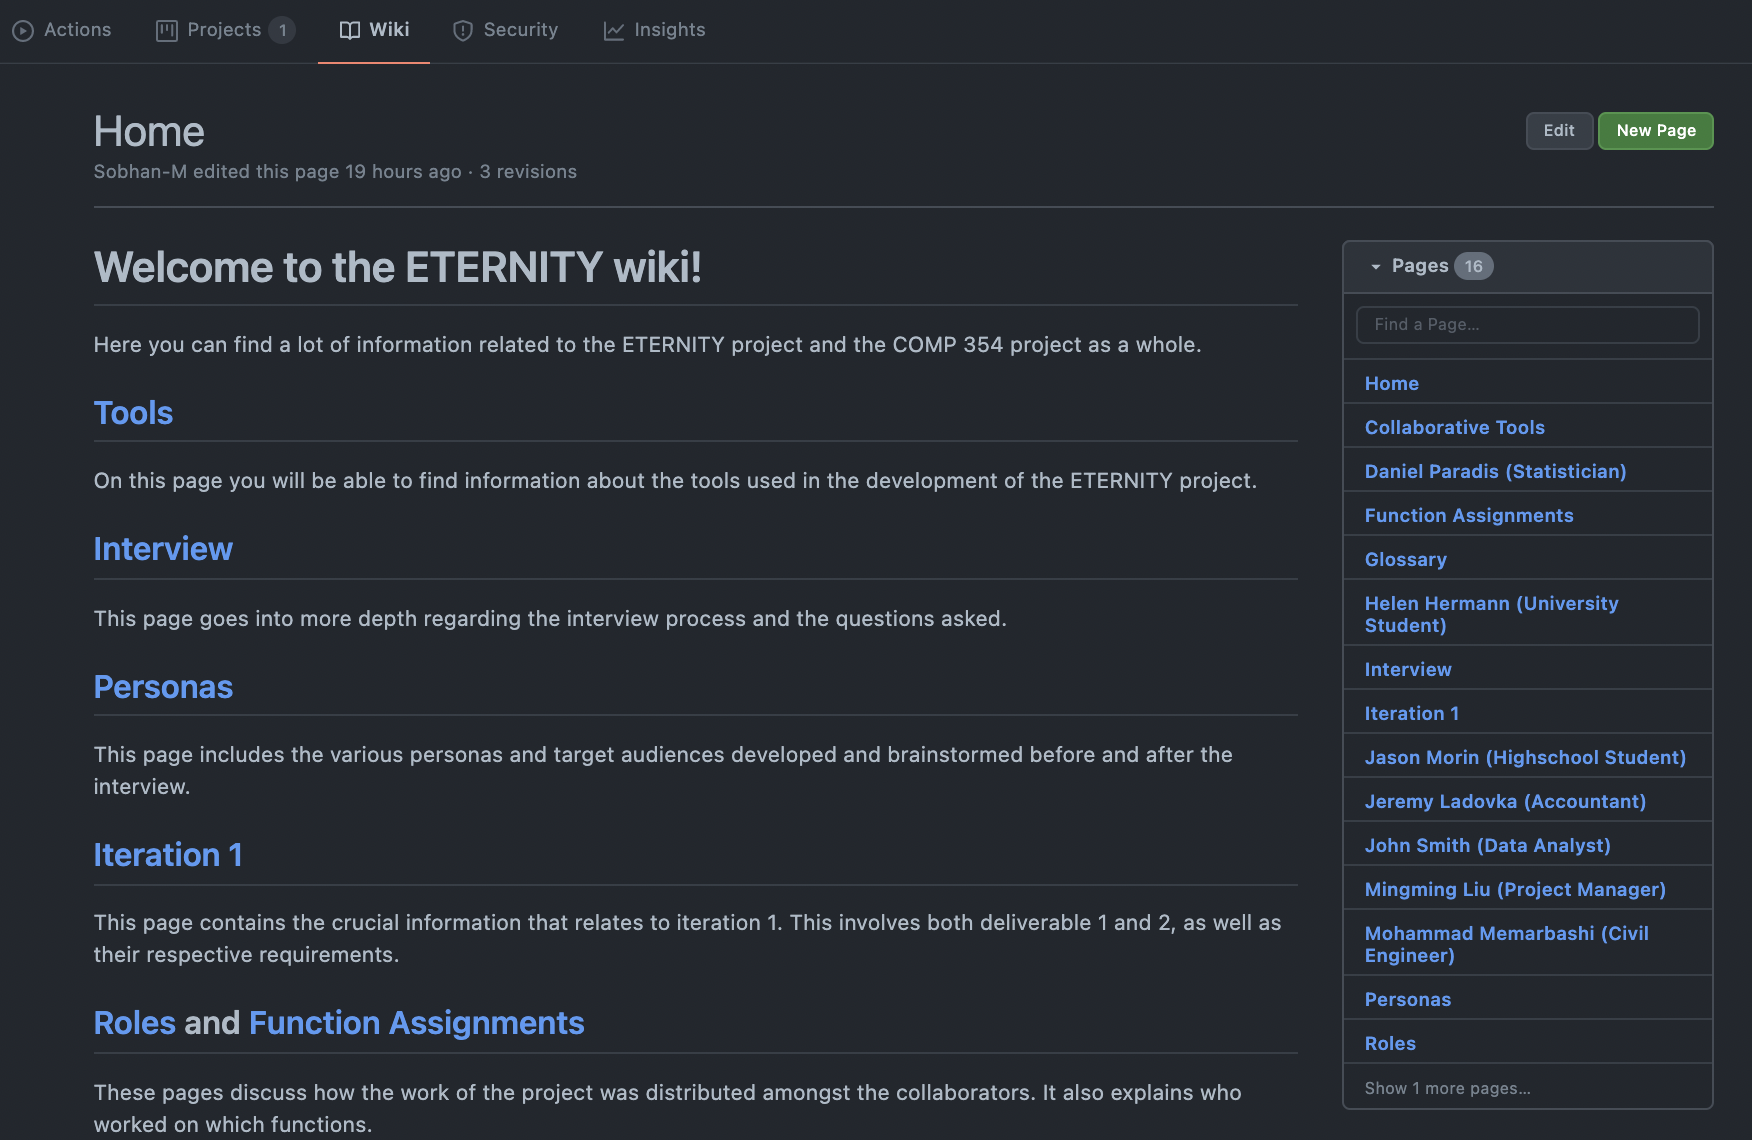
\includegraphics[height=.8\textheight]{wiki.png}
\end{frame}
\end{center}

\begin{frame}
    \frametitle{Interview Process}
    Choosing interviewees:
    \begin{itemize}
        \item Tried to get a variety of interviewees based on whom we thought would be interested in using a calculator
        \item Total of 7 interviewees, one interview conducted by each team member
    \end{itemize}
\end{frame}

\begin{frame}
    \frametitle{Notes about interviews}

    % Maybe mention that, although a calculator is a simple program, there were a lot of things we didn't really consider
    \begin{itemize}
        % A lot of people seem to want customizability. 
        % Also, it makes sense since calculators are pretty similar, so changing the appearance or whatever 
        % makes it kind of unique.
        \item Customizability \pause
        \item People prefer formal notation,\\ i.e. $x^y$ vs x\ \^\ y \pause %idk how to write this without the spaces
        \item There exists a few popular online calculators/ tools with advanced features \\
            i.e. \textit{Wolframe Alpha, Symbolab, Desmos}
    \end{itemize} 
    
\end{frame}

\begin{frame}
    \frametitle{Notes about interviews}

    \textbf{Example of an idea we didn't consider:} \\
    \textit{Which functions that are generally not on a calculator, would you like to see added?} \\
    ``This is very difficult, maybe some constants could be added, 
    like the gravity constant or the speed of light for our fellow engineer."

\end{frame}

% TODO: Considering removing the "initial brainstorm" phase
\begin{frame}
    \frametitle{Personas}
    7 Initial personas, ranging from a variety of different people and different backgrounds who might 
    contribute to different types of use cases.

    \textbf{Initial brainstorm for target groups:}
    \begin{enumerate}
        \item Students
        \item Statisticians
        \item Data Analysts
        \item Businessmen
        \item Accountants
        \item Engineers
        \item Professors
    \end{enumerate}
    
\end{frame}

\begin{frame}
    \frametitle{Personas}

    \textbf{Actual target groups we ended up having:}
    \begin{enumerate}
        \item Highschool Student
        \item University Student
        \item Statisticians
        \item Data Analyst
        \item Accountants
        \item Engineer (Program Manager)
        \item Engineer (Civil Engineer)
    \end{enumerate}
    
\end{frame}

\begin{frame}
    \frametitle{Personas}
    Using the interview responses, we come up with positive and negative personas by first writing up
    a basic bio to make it seem more ``real".
    \begin{itemize}
        \item Then build a table with the important information
    \end{itemize}
\end{frame}

\begin{frame}
    \frametitle{Persona for the target group ``Highschool Student"}
    \begin{tabular}{ |c|c| } 
        \hline
        Name                          & Jason Morin                          \\ \hline
        Gender and age                & male, 15                             \\ \hline
        Disabilities and restrictions & none                                 \\ \hline
        Education                     & Current highschool student           \\ \hline
        Profession                    & Student                              \\ \hline
        Hobbies                       & Building (customizing) computers,    \\ 
                                      & video games, watching Netflix        \\ \hline
        Location of use               & home                                 \\ \hline
                                      & Is very comfortable using computers, \\
        Computer literacy             & and a fast learner for new programs/ \\
                                      & tools but not a power user.          \\ \hline
        Computer environment          & \textit{Google Chrome 91.0.4472.77}  \\ 
                                      & on \textit{Windows 10}               \\ \hline
        Internet literacy             & High, self-taught and fast learner   \\ \hline
    \end{tabular}
\end{frame}


\section{Conclusion}

\begin{frame}
    \frametitle{Persona for the target group ``Accountant"}
    \begin{tabular}{ |c|c| } 
        \hline
        Name                          & Jeremy Ladovka \\ \hline
        Gender and age                & male, 38 \\ \hline
        Disabilities and restrictions & none \\ \hline
        Education                     & Masters, Accountancy \\ \hline
        Profession                    & Accountant \\ \hline
                                      & Math, Soccer, watching movies, \\ 
        Hobbies                       & playing video games, going out \\
                                      & with friends \\ \hline
        Location of use               & Office/ Home (Covid-19) \\ \hline
                                      & Very strong computer skills. \\
        Computer literacy             & Uses computers on a daily basis \\ 
                                      & to perform both work related \\
                                      & tasks and personal hobbies. \\ \hline
        Computer environment          & \textit{Safari v14.1, Mac OS} \\ \hline
        Internet literacy             & High, communicates via Internet daily \\ \hline
    \end{tabular}
\end{frame}



\begin{frame}
    \frametitle{Use Cases}
\begin{columns}
    \column{.5\textwidth}
    \textbf{High Level}
    \begin{itemize}
        \item Validate Calculations Of Other Software
        \item Solve School Assignments
        \item Analyze Sale Statistics
        \item Estimate Cost Of Engineering Projects
        \item Calculate Shopping Expenditures
        \item Help During Exams
        \item Analyze Biology Lab Results
        \item Graph Mathematical Functions
        \item Analyze Large Data Sets
        \item Design Building Architecture
    \end{itemize} \pause
    \column{.5\textwidth}
    \textbf{Low Level}
    \begin{itemize}
        \item Input Data Set
        \item Input Number
        \item Input Function
        \item Input Operator
        \item Graph Function
        \item Calculate Result
        \item Display Result
        \item Clear Result
        \item Modify Colour
    \end{itemize}
    \vspace{2cm}
\end{columns}
\end{frame}

\begin{frame}
    \begin{center}
    \frametitle{Closing Statements}
    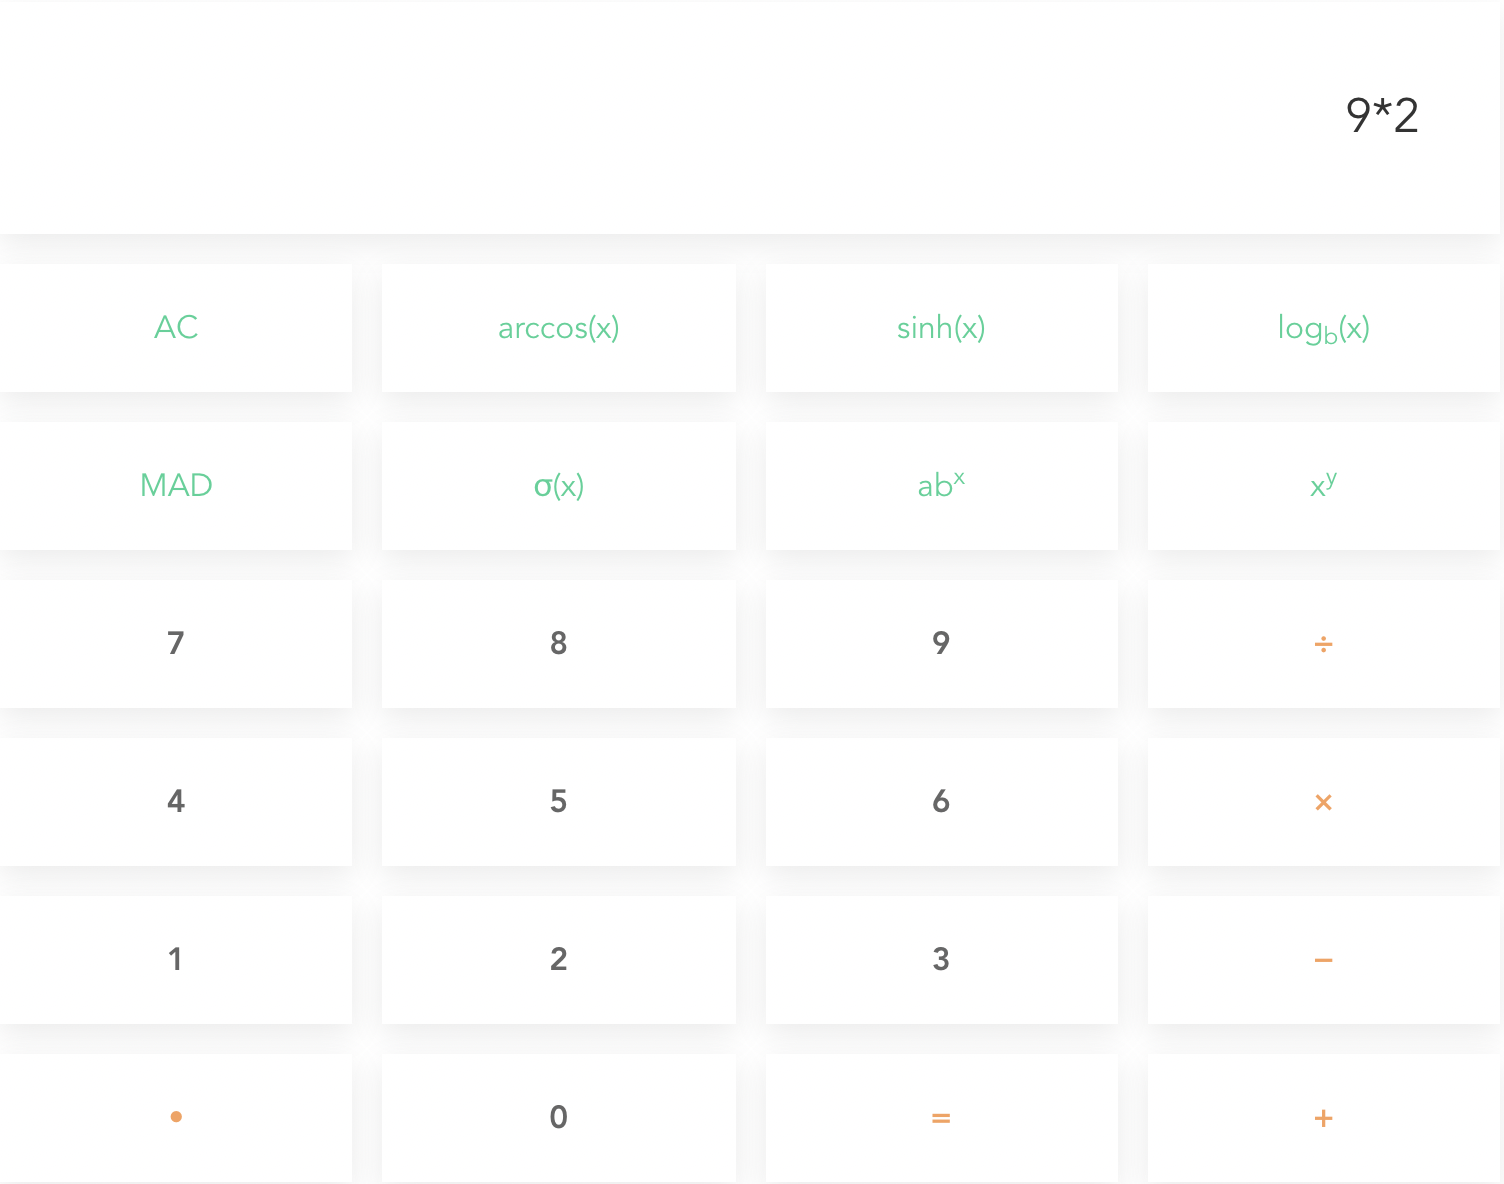
\includegraphics[width=.85\linewidth]{calc.png}
    \end{center}
\end{frame}
\end{document}

